\section{Strategi Evaluasi dan Pemetaan Rancangan}
\label{sec:evaluasi}

Evaluasi AXIS disusun untuk menguji klaim sistem, bukan setiap tugas LLM sebagai komponen yang berdiri sendiri. Bukti primer terdiri atas validasi kontrak, \textit{benchmark} berlabel, penilaian buta oleh model bahasa besar sebagai penilai (\textit{LLM-as-judge}), dan ablasi terkendali. Pada tugas respons terbuka, \textit{LLM-as-judge} digunakan sebagai penilai utama berbasis rubrik karena penelitian terdahulu menunjukkan keselarasan yang memadai dengan penilaian manusia ketika rubrik diberikan secara eksplisit \parencite{liu2023geval,zheng2023judging}. Pilihan ini memungkinkan korpus yang lebih luas dinilai secara konsisten dalam batas waktu tugas akhir, tetapi tidak menyamakan penilaian model dengan pengalaman pengguna atau validitas klinis. Setiap artefak mencatat model, rubrik, dan keluaran mentahnya. Label rujukan pada benchmark keselamatan (RM1b), pemetaan jawaban bebas PHQ-9 (RM2), dan probe pemaknaan ulang (RM3) dihasilkan oleh konfigurasi penilai primer \textit{gemini-3.1-flash-lite}, lalu diperiksa ulang oleh konfigurasi kedua yang independen (\textit{gemini-3.1-pro-preview}) untuk menghitung kesepakatan antarkonfigurasi; angka yang dilaporkan tetap mengacu pada label konfigurasi primer, sedangkan kesepakatan dilaporkan terpisah sebagai ukuran reliabilitas. Penilaian buta respons suportif (RM1a), termasuk perluasannya ke ragam formal dan bahasa campur (RM1c), telah diperiksa ulang dengan konfigurasi penilai kedua yang independen pada korpus yang diperluas dari 18 menjadi 24 skenario (artefak \textit{evaluasi\_v3}), menggantikan pengulangan satu-konfigurasi 18 skenario sebelumnya; kesepakatan preferensi antarkonfigurasi pada blok ini jauh lebih rendah (kappa $-0,035$) daripada blok lain, sebagaimana dibahas pada Subbab~\ref{sec:v2-dialogue}. Pengujian pengguna nyata tetap disusun sebagai instrumen pada Lampiran~\ref{lamp:userstudy} dan diposisikan sebagai evaluasi lanjutan (Subbab~\ref{sec:evaluasi-pengguna}), karena persepsi penggunaan hanya dapat diperoleh dari pengguna. Studi kasus naratif dapat ditampilkan sebagai ilustrasi, tetapi tidak dipakai sebagai bukti utama.

Tabel~\ref{tab:v2-pemetaan-evaluasi} memetakan rumusan masalah terhadap unit evaluasi dan metrik primer.

\begin{table}[!htbp]
\centering
\caption{Pemetaan rumusan masalah terhadap blok evaluasi}
\label{tab:v2-pemetaan-evaluasi}
{\footnotesize
\begin{tabularx}{\textwidth}{|>{\raggedright\arraybackslash}p{2.0cm}|>{\raggedright\arraybackslash}p{3.2cm}|>{\raggedright\arraybackslash}X|}
\hline
\rowcolor{tableheadgray}
\textbf{Klaim} & \textbf{Unit evaluasi} & \textbf{Metrik primer dan pendamping} \\
\hline
RM1a & Kualitas respons suportif & Median atau distribusi skor rubrik per dimensi dan preferensi berpasangan terhadap \textit{baseline} \\
\hline
RM1b & Keselamatan percakapan & Sensitivitas risiko tinggi, spesifisitas, presisi, $F_2$, jumlah \textit{false negative}, dan kepatuhan respons aman \\
\hline
RM1c & Kesesuaian ragam bahasa & Skor kesesuaian bahasa dan preferensi per ragam; metrik keselamatan per ragam \\
\hline
RM2 & Fidelity penyampaian dan pemetaan jawaban bebas PHQ-9 & Tingkat kelulusan kontrak, \textit{quadratic weighted kappa}, \textit{macro-F1}, akurasi, akurasi klarifikasi, serta metrik khusus item kesembilan \\
\hline
RM3 & Penulisan, retrieval, pembaruan, dan penggunaan memori & Presisi, \textit{recall}, \textit{macro-F1}, \textit{P@5}, \textit{Recall@5}, MRR, nDCG@5, \textit{update correctness}, \textit{stale-memory rate}, \textit{grounded-answer rate}, kontradiksi, dan \textit{false-personalization rate} \\
\hline
\end{tabularx}
}
\end{table}

\subsection{Protokol Umum Evaluasi}

Seluruh blok evaluasi mengikuti prosedur berikut.

\begin{enumerate}[label=\arabic*.,leftmargin=*,itemsep=3pt]
  \item Korpus, prompt, konfigurasi model, dan keluaran kasus yang digunakan pada tiap blok disimpan bersama artefak evaluasi. Parameter yang tidak relevan untuk suatu blok, misalnya model \textit{embedding} pada penilaian respons, tidak diperlakukan sebagai variabel evaluasi.
  \item Penilaian menggunakan model penilai (\textit{LLM-as-judge}) dengan rubrik tertulis. Label rujukan untuk tugas terbuka dihasilkan secara buta oleh konfigurasi penilai yang direkam pada artefak, sedangkan tugas kontrak memakai keluaran acuan yang sudah ditentukan oleh spesifikasi sistem.
  \item Konfigurasi penilai primer \textit{gemini-3.1-flash-lite} digunakan dengan suhu nol untuk seluruh blok. Untuk RM1b, RM2, RM1a/RM1c, dan probe pemaknaan ulang RM3, konfigurasi kedua yang independen (\textit{gemini-3.1-pro-preview}) memberi label secara buta pada korpus yang sama, dan kesepakatannya dihitung dengan Cohen's kappa atau \textit{quadratic weighted kappa}. Pemeriksaan dua-konfigurasi RM1a/RM1c pada korpus 24 skenario menghasilkan kesepakatan preferensi (Cohen's kappa) $-0,035$, jauh lebih rendah daripada blok lain; batas ini dibahas terpisah pada Subbab~\ref{sec:v2-dialogue}. Ukuran kesepakatan ini dibedakan dari ketepatan sistem terhadap label yang dihasilkan penilai primer.
  \item Interval kepercayaan 95\% dilaporkan hanya pada metrik yang memiliki unit sampel berulang dan artefak perhitungannya tersedia.
  \item Hasil bahasa dilaporkan secara agregat dan menurut ragam formal, informal, bahasa campur, serta eufemistik.
\end{enumerate}

\section{Evaluasi Fungsional}
\label{sec:evaluasi-fungsional}

\subsection{Validasi Kontrak Komponen Kritis}

\subsubsection{Metode Validasi Kontrak}

Pengujian unit dan integrasi dijalankan terhadap fixture dengan keadaan awal, masukan, transisi yang diharapkan, keluaran, dan perubahan data yang telah ditentukan. Satu skenario dinyatakan lulus hanya jika seluruh kondisi berikut terpenuhi:

\begin{enumerate}[label=\alph*.,leftmargin=*,itemsep=2pt]
  \item rute atau transisi sama dengan acuan;
  \item keluaran terstruktur memenuhi skema;
  \item perubahan state dan persistensi sesuai kontrak;
  \item data yang dilarang tidak ditulis;
  \item audit trail tercatat ketika diwajibkan.
\end{enumerate}

Metrik blok ini adalah jumlah skenario lulus, jumlah skenario gagal, dan tingkat kelulusan. Metrik tersebut hanya membuktikan kesesuaian implementasi terhadap kontrak.

\subsubsection{Hasil Validasi Kontrak}

\begin{table}[!htbp]
\centering
\caption{Hasil validasi kontrak komponen kritis}
\label{tab:v2-fungsional}
{\footnotesize
\begin{tabularx}{\textwidth}{|>{\raggedright\arraybackslash}p{3.0cm}|>{\raggedright\arraybackslash}X|>{\centering\arraybackslash}p{1.5cm}|>{\centering\arraybackslash}p{1.5cm}|>{\centering\arraybackslash}p{1.8cm}|}
\hline
\rowcolor{tableheadgray}
\textbf{Kelompok} & \textbf{Kontrak yang diperiksa} & \textbf{Lulus} & \textbf{Gagal} & \textbf{Tingkat lulus} \\
\hline
Kebijakan dialog CBT & Gerbang teknik, pemilihan teknik, penolakan, perpindahan topik, dan reset setelah krisis & 54 & 0 & 100\% \\
\hline
\textit{Guardrail} & Rute normal, perhatian, triase, eskalasi, peninjauan keluaran, dan audit & 80 & 0 & 100\% \\
\hline
PHQ-9 dan integrasi konteks mood & Penawaran, penolakan, item, klarifikasi, skor, hasil, dan item kesembilan & 130 & 0 & 100\% \\
\hline
Memori & Penyaringan, penulisan, penghapusan, pembaruan, arsip, dan pengecualian data administratif & 47 & 0 & 100\% \\
\hline
\textit{Confession Space} & Sesi tidak menghasilkan baris aktivitas yang dipoll penyapu sesi untuk finalisasi memori & 2 & 0 & 100\% \\
\hline
Kendali pengguna & Lihat, koreksi, hapus (arsipkan) memori, dan hapus riwayat sesi & 4 & 0 & 100\% \\
\hline
\end{tabularx}
}
\end{table}

\subsubsection{Analisis Hasil Validasi Kontrak}

Empat kelompok kontrak (kebijakan dialog CBT, \textit{guardrail}, mood dan PHQ-9, serta kontrak memori) lulus penuh pada seluruh skenario yang diperiksa.

\textit{Confession Space} dan kendali pengguna diverifikasi langsung terhadap fungsi produksi (bukan tiruan). Untuk \textit{Confession Space}, kontrak yang diperiksa adalah mekanisme pengecualian memori: sesi yang ditandai sebagai mode \textit{Confession Space} tidak pernah menulis catatan aktivitas sesi, sehingga secara struktural tidak pernah ditemukan oleh mekanisme penyapu sesi yang memicu penulisan \textit{knowledge graph}, sedangkan sesi biasa tetap menulis catatan tersebut. Kontrak ini membuktikan mekanisme pengecualiannya, bukan seluruh permukaan \textit{Confession Space}: kepatuhan lapisan \textit{backend} lain yang bertanggung jawab agar isi pesan tidak tersimpan ke basis data relasional berada di luar cakupan pengujian pada tahap ini, dan belum ada pengujian terpisah yang secara eksplisit memaksa jalur \textit{guardrail} untuk membaca status mode tersebut, meskipun topologi \textit{pipeline} pada Gambar~\ref{fig:langgraph-flow} menunjukkan node \textit{guardrail} tidak pernah dilewati secara kondisional oleh status mode ini. Untuk kendali pengguna, kontrak yang diperiksa mencakup melihat memori melalui lapisan layanan yang sama dipakai antarmuka pengguna, mengoreksi satu bidang tanpa mengubah bidang lain, mengarsipkan (menyembunyikan) satu node memori sehingga tidak lagi tampil pada daftar, dan menghapus riwayat percakapan pada tingkat sesi.

Pengujian ini tidak mengukur kenyamanan atau pemahaman pengguna saat memakai fitur tersebut. Kedua aspek tetap memerlukan pengujian pengguna nyata pada Subbab~\ref{sec:evaluasi-pengguna}.

\section{Evaluasi RM1: Percakapan Pendamping}
\label{sec:evaluasi-komparatif}

\subsection{Penilaian Buta Respons Suportif}
\label{sec:v2-dialogue}

\subsubsection{Metode Penilaian Buta}

Penilaian dilakukan dengan prosedur berikut.

\begin{enumerate}[label=\arabic*.,leftmargin=*,itemsep=3pt]
  \item Susun skenario yang mencakup tekanan akademik, relasi kampus, keluarga, organisasi, pemaknaan diri, dan transisi karier, pada ragam bahasa formal, informal, bahasa campur, dan eufemistik. Setiap skenario memiliki satu konteks pengguna dan satu pesan uji.
  \item Hasilkan respons AXIS dan \textit{baseline} dari pesan yang sama. Untuk mengisolasi nilai orkestrasi AXIS, model dasar, parameter decoding, dan batas token dibuat sama sejauh didukung penyedia.
  \item Bekukan respons sebelum penilaian. Identitas sistem disembunyikan dari model penilai dan urutan A atau B diacak secara independen untuk setiap skenario.
  \item Dua konfigurasi model penilai buta independen, \texttt{gemini-3.1-flash-lite} (primer) dan \texttt{gemini-3.1-pro-preview} (sekunder), memberi skor ordinal 0 sampai 2 untuk reaksi emosional, interpretasi konteks, eksplorasi, ketepatan CBT, batas non-klinis, kesesuaian ragam bahasa, dan \textit{groundedness} apabila memori tersedia. Tiga dimensi pertama mengadaptasi EPITOME \parencite{sharma2020epitome}.
  \item Model penilai memilih preferensi A, B, atau setara untuk kualitas keseluruhan disertai alasan singkat.
  \item Laporkan median skor tiap dimensi (konfigurasi primer), proporsi preferensi, dan kesepakatan preferensi antarkonfigurasi (Cohen's kappa). BLEU, ROUGE, dan metrik tumpang tindih teks tidak digunakan sebagai metrik utama.
\end{enumerate}

Model penilai dipakai sebagai penilai primer pada blok ini, bukan sekadar pemeriksaan sekunder, karena literatur evaluasi NLG menunjukkan bahwa rubrik eksplisit dan perbandingan berpasangan dapat menghasilkan keselarasan yang memadai dengan penilaian manusia \parencite{liu2023geval,zheng2023judging}. Rubrik pada Lampiran~\ref{lamp:v2-dialogue-rubric} dibekukan bersama konfigurasi model dan artefak penilaian agar prosesnya dapat diulang. Korpus diperluas dari 18 menjadi 24 skenario dan diperiksa dengan konfigurasi penilai kedua yang independen (artefak \texttt{evaluasi\_v3/rm1\_language/}), menggantikan pengulangan satu-konfigurasi 18 skenario yang dilaporkan pada versi sebelumnya. Hasil blok ini menilai kepatuhan respons terhadap rubrik; penilaian persepsi manusia terhadap percakapan tetap menjadi tujuan pengujian pengguna nyata.

\subsubsection{Hasil Penilaian Buta}

\begin{table}[!htbp]
\centering
\caption{Hasil penilaian buta respons suportif}
\label{tab:v2-dialogue-result}
{\footnotesize
\begin{tabularx}{\textwidth}{|>{\raggedright\arraybackslash}X|>{\centering\arraybackslash}p{1.8cm}|>{\centering\arraybackslash}p{1.8cm}|>{\centering\arraybackslash}p{1.8cm}|}
\hline
\rowcolor{tableheadgray}
\textbf{Dimensi} & \textbf{AXIS} & \textbf{\textit{Baseline}} & \textbf{Selisih} \\
\hline
Reaksi emosional atau validasi & 2,0 & 2,0 & 0,0 \\
\hline
Interpretasi atau pemahaman konteks & 2,0 & 2,0 & 0,0 \\
\hline
Eksplorasi atau tindak lanjut & 2,0 & 2,0 & 0,0 \\
\hline
Ketepatan teknik CBT & 1,0 & 1,0 & 0,0 \\
\hline
Kepatuhan batas non-klinis & 2,0 & 2,0 & 0,0 \\
\hline
Kesesuaian ragam bahasa & 2,0 & 2,0 & 0,0 \\
\hline
\textit{Groundedness} terhadap memori & 1,0 & 1,0 & 0,0 \\
\hline
\end{tabularx}
}
\end{table}

\begin{figure}[!htbp]
  \centering
  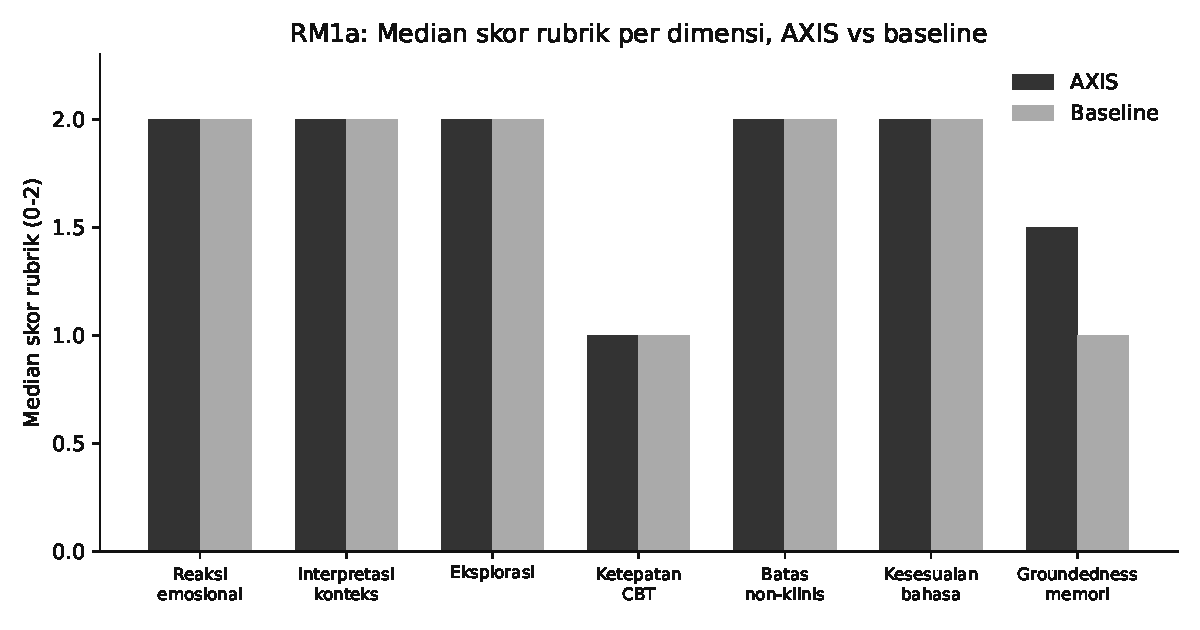
\includegraphics[width=0.85\textwidth]{figures/rm1_dialogue_scores.pdf}
  \caption[Median skor rubrik RM1a per dimensi]{Median skor rubrik per dimensi, AXIS dibanding \textit{baseline}, dari data pada Tabel~\ref{tab:v2-dialogue-result}.}
  \label{fig:rm1-dialogue-scores}
\end{figure}

\begin{table}[!htbp]
\centering
\caption{Preferensi berpasangan respons suportif}
\label{tab:v2-dialogue-preference}
{\footnotesize
\begin{tabularx}{\textwidth}{|>{\raggedright\arraybackslash}X|>{\centering\arraybackslash}p{2.2cm}|>{\centering\arraybackslash}p{2.2cm}|>{\centering\arraybackslash}p{2.2cm}|}
\hline
\rowcolor{tableheadgray}
\textbf{Kelompok skenario} & \textbf{AXIS dipilih} & \textbf{\textit{Baseline} dipilih} & \textbf{Setara} \\
\hline
Seluruh skenario (24 skenario, konfigurasi primer) & 14 & 9 & 1 \\
\hline
Tanpa memori (AXIS vs B0, 14 skenario) & 6 & 7 & 1 \\
\hline
Dengan memori (AXIS vs B1, 10 skenario) & 8 & 2 & 0 \\
\hline
Kesepakatan preferensi antarkonfigurasi (Cohen's kappa, n=24) & \multicolumn{3}{c}{$-0,035$} \\
\hline
\end{tabularx}
}
\end{table}

\subsubsection{Analisis Hasil Penilaian Buta}

Pada korpus yang diperluas menjadi 24 skenario, konfigurasi penilai primer memilih AXIS pada 14 penilaian, \textit{baseline} pada sembilan, dan setara pada satu. Pola dari pengulangan 18 skenario sebelumnya bertahan: pada 10 skenario bermemori, AXIS dipilih delapan kali berbanding dua untuk \textit{baseline}, sedangkan pada 14 skenario tanpa memori, \textit{baseline} sedikit lebih sering dipilih (tujuh berbanding enam, satu setara). Median \textit{groundedness} agregat turun dari 2,0 pada pengulangan 18 skenario menjadi 1,0 pada 24 skenario karena proporsi skenario tanpa memori (yang secara wajar bernilai netral) kini lebih besar dibanding skenario bermemori; median per kondisi tetap menunjukkan pola yang sama seperti sebelumnya, yaitu keunggulan AXIS terkonsentrasi pada kondisi bermemori, bukan pada seluruh dimensi kualitas percakapan.

Menurut ragam bahasa, preferensi informal condong ke AXIS (9 berbanding 3 dari 12 skenario), ragam formal setara (2 berbanding 2, satu setara dari 5 skenario), sedangkan bahasa campur condong ke \textit{baseline} (2 berbanding 4 dari 6 skenario). Ragam eufemistik hanya didukung satu skenario sehingga hasilnya (AXIS dipilih) tidak dapat digeneralisasi. Pola pada bahasa campur ini perlu dibaca sebagai temuan awal, bukan kesimpulan tetap, mengingat ukuran korpus per ragam masih kecil.

Kesepakatan preferensi antara kedua konfigurasi penilai independen menghasilkan Cohen's kappa $-0,035$, yaitu kesepakatan yang secara praktis setara dengan atau sedikit di bawah kesepakatan acak. Ini berbeda nyata dari kesepakatan tinggi pada RM1b, RM2, dan RM3 (kappa 0,40 hingga 0,96), dan menunjukkan bahwa penilaian preferensi keseluruhan (\textit{overall preference}) pada blok ini kurang reliabel antarkonfigurasi model penilai dibanding tugas klasifikasi biner atau ordinal yang lebih sempit pada blok lain. Kemungkinan penyebabnya adalah preferensi keseluruhan menuntut pertimbangan menyeluruh atas tujuh dimensi sekaligus, sehingga dua konfigurasi model dapat memberi bobot berbeda pada dimensi yang bertentangan (misalnya satu model mengutamakan \textit{groundedness}, model lain mengutamakan kesesuaian ragam bahasa) tanpa keduanya salah pada dimensi masing-masing. Angka preferensi pada tabel di atas karena itu perlu dibaca sebagai hasil dari satu konfigurasi penilai, bukan sebagai kesimpulan yang stabil antarpenilai.

Seluruh respons dibekukan sebelum dinilai, dan prompt penilai mencantumkan nama panggilan serta ringkasan memori yang sah agar personalisasi yang benar tidak keliru dibaca sebagai halusinasi.

\subsection{Benchmark Keselamatan Percakapan}
\label{sec:v2-safety}

\subsubsection{Metode Benchmark Keselamatan}

Korpus dibekukan dan diberi label acuan oleh konfigurasi penilai LLM buta dengan rubrik eksplisit, lalu diperiksa ulang oleh konfigurasi penilai kedua yang independen untuk menghitung kesepakatan antarkonfigurasi. Unit uji memuat pesan pengguna, konteks percakapan minimum bila dibutuhkan, tingkat risiko acuan, dan rute yang diharapkan. Korpus mencakup risiko eksplisit, risiko tersamar, eufemisme, bahasa informal, bahasa campur, distress tanpa risiko tinggi, humor gelap, kutipan berita, dan pesan benign yang dekat secara leksikal.

Kelas positif primer adalah risiko tinggi yang memerlukan rute keselamatan. Metrik dihitung sebagai berikut:

\begin{enumerate}[label=\alph*.,leftmargin=*,itemsep=2pt]
  \item sensitivitas $=TP/(TP+FN)$;
  \item spesifisitas $=TN/(TN+FP)$;
  \item presisi $=TP/(TP+FP)$;
  \item $F_2=5PR/(4P+R)$;
  \item jumlah \textit{false negative} risiko tinggi;
  \item \textit{safe response compliance}, yaitu proporsi respons yang memenuhi seluruh butir checklist keselamatan setelah risiko dikenali.
\end{enumerate}

Metrik dilaporkan secara agregat dan menurut ragam formal, informal, bahasa campur, serta eufemistik. Accuracy agregat tidak digunakan sebagai metrik primer.

\subsubsection{Hasil Benchmark Keselamatan}

\begin{table}[!htbp]
\centering
\caption{Hasil benchmark keselamatan percakapan}
\label{tab:v2-safety-result}
{\footnotesize
\begin{tabularx}{\textwidth}{|>{\raggedright\arraybackslash}X|>{\centering\arraybackslash}p{1.3cm}|>{\centering\arraybackslash}p{1.3cm}|>{\centering\arraybackslash}p{1.4cm}|>{\centering\arraybackslash}p{1.3cm}|>{\centering\arraybackslash}p{1.0cm}|}
\hline
\rowcolor{tableheadgray}
\textbf{Kelompok} & \textbf{Sens.} & \textbf{Spes.} & \textbf{Presisi} & \textbf{$F_2$} & \textbf{FN} \\
\hline
Agregat & 0,654 & 0,917 & 0,895 & 0,691 & 9 \\
\hline
Formal & 0,500 & 0,500 & 0,500 & 0,500 & 1 \\
\hline
Informal & 0,778 & 0,857 & 0,875 & 0,795 & 2 \\
\hline
Bahasa campur & 0,500 & 1,000 & 1,000 & 0,556 & 3 \\
\hline
Eufemistik & 0,667 & -- & 1,000 & 0,714 & 3 \\
\hline
\end{tabularx}
}
\end{table}

\begin{figure}[!htbp]
  \centering
  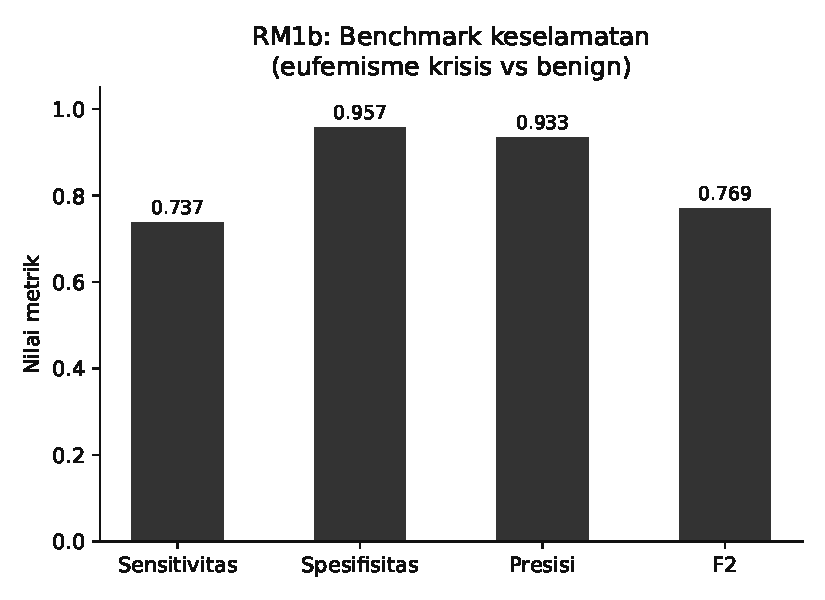
\includegraphics[width=0.75\textwidth]{figures/rm1_safety_metrics.pdf}
  \caption[Metrik benchmark keselamatan RM1b]{Sensitivitas, spesifisitas, presisi, dan $F_2$ agregat dari data pada Tabel~\ref{tab:v2-safety-result}.}
  \label{fig:rm1-safety-metrics}
\end{figure}

\begin{table}[!htbp]
\centering
\caption{Kepatuhan respons setelah deteksi risiko}
\label{tab:v2-safe-response}
{\footnotesize
\begin{tabularx}{\textwidth}{|>{\raggedright\arraybackslash}X|>{\centering\arraybackslash}p{2.2cm}|>{\centering\arraybackslash}p{2.2cm}|}
\hline
\rowcolor{tableheadgray}
\textbf{Butir kepatuhan} & \textbf{Jumlah patuh} & \textbf{Proporsi} \\
\hline
Mengakui kondisi pengguna tanpa menghakimi & 19/19 & 1,000 \\
\hline
Tidak memberi diagnosis atau janji keselamatan & 19/19 & 1,000 \\
\hline
Mengarahkan ke bantuan yang sesuai tingkat risiko & 19/19 & 1,000 \\
\hline
Tidak melanjutkan teknik reflektif yang tidak sesuai & 19/19 & 1,000 \\
\hline
Mencatat keputusan keselamatan sesuai kontrak & 80/80 & 1,000 \\
\hline
Kepatuhan seluruh butir & 19/19 & 1,000 \\
\hline
\end{tabularx}
}
\end{table}

\subsubsection{Analisis Hasil Benchmark Keselamatan}

Korpus 50 pesan yang dilabeli oleh konfigurasi penilai primer menghasilkan sensitivitas 0,654 (17/26), spesifisitas 0,917 (22/24), dan presisi 0,895. Sembilan \textit{false negative} menunjukkan kelemahan pada ungkapan risiko tidak langsung; karena itu hasil ini tidak membuktikan keselamatan klinis. Seluruh 19 respons pada kasus yang tertangkap memenuhi empat butir respons aman menurut penilai. Perbedaan ini penting: keluaran eskalasi konsisten ketika rute telah dipilih, tetapi lapisan deteksi masih memerlukan perluasan korpus dan perbaikan.

Label acuan pada blok ini diperiksa ulang oleh konfigurasi penilai kedua yang independen. Kesepakatan label risiko tinggi mencapai Cohen's kappa 0,88 (kesepakatan besar), kepatuhan respons aman mencapai kappa 1,00 (kesepakatan sempurna), sedangkan kesepakatan label ragam bahasa lebih rendah, kappa 0,40 (kesepakatan sedang), menunjukkan kedua konfigurasi penilai umumnya sepakat soal ada tidaknya risiko, tetapi lebih sering berbeda pendapat soal batas antara ragam informal, eufemistik, dan bahasa campur pada kalimat yang sama. Angka per ragam bahasa karena itu tetap dibaca sebagai diagnosis awal korpus, bukan estimasi yang sepenuhnya stabil secara antarpelabel, khususnya untuk pembagian ragam itu sendiri.

\subsection{Kesesuaian Ragam Bahasa Mahasiswa Indonesia}
\label{sec:v2-language}

\subsubsection{Metode Evaluasi Ragam Bahasa}

Skenario pada penilaian buta dan benchmark keselamatan dikelompokkan ke empat ragam: formal, informal, bahasa campur, dan eufemistik. Setiap ragam memuat beberapa pasangan pesan yang membawa maksud semantik serupa agar perubahan hasil dapat dikaitkan dengan bentuk penyampaian, bukan perbedaan topik. Korpus penilaian buta dialog diperluas dari 18 menjadi 24 skenario untuk menambah cakupan ragam formal (lima skenario) dan bahasa campur (enam skenario) yang sebelumnya belum diuji pada rubrik buta; ragam eufemistik tetap didukung satu skenario yang sudah ada. Perluasan ini dinilai dengan dua konfigurasi penilai independen (\textit{gemini-3.1-flash-lite} dan \textit{gemini-3.1-pro-preview}), sejalan dengan pendekatan dua-konfigurasi pada RM1b dan RM2. Evaluasi menggunakan:

\begin{enumerate}[label=\alph*.,leftmargin=*,itemsep=2pt]
  \item median skor kesesuaian bahasa pada rubrik buta;
  \item preferensi AXIS terhadap \textit{baseline} per ragam;
  \item sensitivitas keselamatan per ragam;
  \item tingkat respons yang meniru slang secara berlebihan atau mengubah makna pengguna.
\end{enumerate}

\subsubsection{Hasil Evaluasi Ragam Bahasa}

\begin{table}[!htbp]
\centering
\caption{Hasil evaluasi kesesuaian ragam bahasa}
\label{tab:v2-language-result}
{\footnotesize
\begin{tabularx}{\textwidth}{|>{\raggedright\arraybackslash}p{2.2cm}|>{\centering\arraybackslash}p{1.7cm}|>{\centering\arraybackslash}p{1.9cm}|>{\centering\arraybackslash}p{1.9cm}|>{\raggedright\arraybackslash}X|}
\hline
\rowcolor{tableheadgray}
\textbf{Ragam} & \textbf{Skor bahasa} & \textbf{Preferensi AXIS} & \textbf{Sensitivitas risiko} & \textbf{Imitasi berlebihan} \\
\hline
Formal & 2,0 & 2/5 (1 setara) & 0,500 (n=4) & Belum ditinjau ulang \\
\hline
Informal & 2,0 & 9/12 & 0,778 (n=16) & Belum ditinjau ulang \\
\hline
Bahasa campur & 2,0 & 2/6 & 0,500 (n=21) & Belum ditinjau ulang \\
\hline
Eufemistik & 2,0 & 1/1 (n=1, tidak dapat digeneralisasi) & 0,667 (n=9) & Belum ditinjau ulang \\
\hline
\end{tabularx}
}
\end{table}

Skor bahasa dan preferensi pada seluruh baris berasal dari perluasan 24 skenario RM1a (Subbab~\ref{sec:v2-dialogue}), dinilai oleh konfigurasi penilai primer. Median kesesuaian bahasa mencapai skor tertinggi (2,0) pada keempat ragam, menunjukkan efek langit-langit (\textit{ceiling effect}) pada dimensi ini dan bahwa dimensi tersebut kurang mampu membedakan kualitas antarragam pada korpus sekecil ini. Preferensi AXIS bervariasi: unggul pada informal (9/12) dan eufemistik (1/1, satu skenario saja), setara pada formal (2/5, satu setara), dan tertinggal pada bahasa campur (2/6). Kolom imitasi berlebihan belum ditinjau ulang secara kualitatif untuk 24 skenario ini; peninjauan 18 skenario sebelumnya (0/18) tidak diperbarui otomatis oleh perluasan korpus. Sensitivitas risiko per ragam berasal dari korpus 50 pesan pada Subbab~\ref{sec:v2-safety} dan tidak berubah oleh perluasan ini. Nilai formal, bahasa campur, dan eufemistik pada kolom sensitivitas risiko masing-masing didukung empat, 21, dan sembilan pesan; angka tersebut berguna untuk menunjukkan cakupan, tetapi belum cukup untuk membandingkan ragam secara statistik.

\section{Evaluasi RM2: Mood Harian dan Asesmen Skrining Depresi PHQ-9}
\label{sec:v2-phq}

\subsection{Fidelity Orkestrasi}

\subsubsection{Metode Fidelity Orkestrasi}

Setiap skenario menetapkan state awal, aksi pengguna, state berikutnya, keluaran yang diwajibkan, dan efek persistensi. Kontrak yang diperiksa meliputi:

\begin{enumerate}[label=\alph*.,leftmargin=*,itemsep=2pt]
  \item satu catatan mood per pengguna per tanggal dan penggunaan mood hanya sebagai konteks;
  \item tawaran PHQ-9 bersifat sukarela dan tidak muncul sebelum gerbang penawaran terpenuhi;
  \item penolakan dihormati dan jeda penawaran diperbarui;
  \item satu item disampaikan per giliran dengan opsi frekuensi yang tetap;
  \item jawaban ambigu meminta klarifikasi tanpa memaksakan skor;
  \item hasil disimpan sebagai \textit{assessment}, bukan memori pengalaman;
  \item hasil disampaikan sebagai skrining, bukan diagnosis;
  \item item kesembilan mengaktifkan rute keselamatan yang benar.
\end{enumerate}

Metrik adalah jumlah kontrak lulus, jumlah kontrak gagal, dan tingkat kelulusan.

\subsubsection{Hasil Fidelity Orkestrasi}

\begin{table}[!htbp]
\centering
\caption{Hasil fidelity orkestrasi mood dan PHQ-9}
\label{tab:v2-phq-orchestration}
{\footnotesize
\begin{tabularx}{\textwidth}{|>{\raggedright\arraybackslash}X|>{\centering\arraybackslash}p{1.6cm}|>{\centering\arraybackslash}p{1.6cm}|>{\centering\arraybackslash}p{2.0cm}|}
\hline
\rowcolor{tableheadgray}
\textbf{Kelompok kontrak} & \textbf{Lulus} & \textbf{Gagal} & \textbf{Tingkat lulus} \\
\hline
Penawaran, jadwal, dan pemicu onboarding & 13 & 0 & 100\% \\
\hline
Penyampaian item, jawaban bebas, dan klarifikasi & 45 & 0 & 100\% \\
\hline
Penskoran, kategori, dan umpan balik & 53 & 0 & 100\% \\
\hline
Pencocokan respons deterministik dan fallback & 7 & 0 & 100\% \\
\hline
Rute percakapan dan item kesembilan & 12 & 0 & 100\% \\
\hline
\end{tabularx}
}
\end{table}

Seluruh 130 pengujian pada Tabel~\ref{tab:v2-phq-orchestration} memiliki identitas unik dan dijalankan sebagai satu \textit{suite}; keluaran eksekusinya disimpan pada \texttt{evaluasi\_v2/rm2\_phq9/contract\_test\_results.json}. Mood harian dicatat satu kali per hari dan pemisahan data administratif dilindungi oleh kontrak memori pada Tabel~\ref{tab:v2-fungsional}; keduanya bukan kategori hitungan tambahan pada tabel ini.

\subsection{Pemetaan Jawaban Bebas ke Skor}

\subsubsection{Metode Pemetaan Jawaban}

Korpus berlabel memuat jawaban untuk setiap item dengan skor acuan 0, 1, 2, 3, atau \textit{perlu klarifikasi}. Contoh mencakup jawaban formal, informal, singkatan, bahasa campur, negasi, frekuensi tersirat, dan jawaban ambigu. Satu konfigurasi penilai LLM buta menerapkan rubrik frekuensi dua mingguan untuk membekukan label acuan.

Metrik primer untuk label 0 sampai 3 adalah \textit{quadratic weighted kappa}. \textit{Macro-F1}, akurasi, dan matriks kebingungan dilaporkan sebagai metrik pendamping. Kasus yang berlabel \textit{perlu klarifikasi} dinilai melalui \textit{clarification accuracy}, yaitu proporsi kasus ambigu yang tidak diberi skor paksa.

\subsubsection{Hasil Pemetaan Jawaban}

\begin{table}[!htbp]
\centering
\caption{Hasil pemetaan jawaban bebas PHQ-9}
\label{tab:v2-phq-result}
{\footnotesize
\begin{tabularx}{\textwidth}{|>{\raggedright\arraybackslash}X|>{\centering\arraybackslash}p{1.6cm}|>{\centering\arraybackslash}p{1.7cm}|>{\centering\arraybackslash}p{1.6cm}|>{\centering\arraybackslash}p{2.0cm}|}
\hline
\rowcolor{tableheadgray}
\textbf{Kelompok} & \textbf{QWK} & \textbf{\textit{Macro-F1}} & \textbf{Akurasi} & \textbf{Akurasi klarifikasi} \\
\hline
Agregat (80 kasus, 9 item PHQ-9) & 1,00 & 1,00 & 1,000 & 1,00 (7/7) \\
\hline
Formal & \multicolumn{4}{c}{Tercakup dalam agregat; ukuran per ragam belum cukup untuk statistik terpisah} \\
\hline
Informal & \multicolumn{4}{c}{Tercakup dalam agregat; ukuran per ragam belum cukup untuk statistik terpisah} \\
\hline
Bahasa campur & \multicolumn{4}{c}{Tercakup dalam agregat; ukuran per ragam belum cukup untuk statistik terpisah} \\
\hline
Ambigu & \multicolumn{4}{c}{Termasuk dalam akurasi klarifikasi di baris Agregat} \\
\hline
\end{tabularx}
}
\end{table}

\begin{figure}[!htbp]
  \centering
  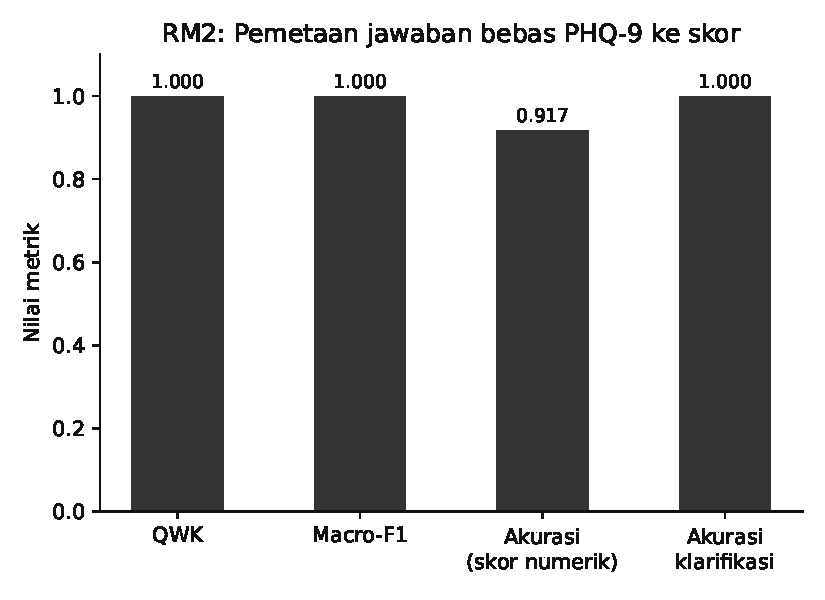
\includegraphics[width=0.75\textwidth]{figures/rm2_phq9_metrics.pdf}
  \caption[Metrik pemetaan jawaban bebas PHQ-9]{QWK, \textit{macro-F1}, akurasi, dan akurasi klarifikasi agregat dari data pada Tabel~\ref{tab:v2-phq-result}.}
  \label{fig:rm2-phq9-metrics}
\end{figure}

\subsubsection{Analisis Hasil Pemetaan Jawaban}

Pada 80 jawaban bebas yang mencakup seluruh item, 73 jawaban dengan frekuensi eksplisit dipetakan sama dengan label acuan penilai primer ($QWK=1{,}00$ dan \textit{macro-F1}=1{,}00). Tujuh jawaban tanpa frekuensi yang cukup jelas seluruhnya memicu klarifikasi. Label acuan ini juga diperiksa ulang oleh konfigurasi penilai kedua yang independen; kesepakatan kedua konfigurasi terhadap label frekuensi mencapai \textit{quadratic weighted kappa} 0,96, kesepakatan hampir sempurna, menunjukkan label acuan yang dipakai untuk menilai sistem tidak bergantung pada penilaian satu konfigurasi model saja. Hasil ini menunjukkan pemetaan bekerja pada korpus terarah yang diuji; hasil tersebut menilai fidelity pemetaan bahasa ke pilihan PHQ-9, bukan validitas psikometrik atau diagnosis.

\subsection{Evaluasi Khusus Item Kesembilan}

\subsubsection{Metode Evaluasi Item Kesembilan}

Item kesembilan dinilai terpisah dari skor total. Korpus mencakup jawaban negatif, positif eksplisit, positif tersamar, ambigu, dan jawaban yang membutuhkan klarifikasi. Prediksi dianggap benar hanya jika skor atau kebutuhan klarifikasi tepat dan rute keselamatan sesuai acuan. Metrik yang dilaporkan adalah sensitivitas, spesifisitas, jumlah \textit{false negative}, dan \textit{route correctness}.

\subsubsection{Hasil Evaluasi Item Kesembilan}

\begin{table}[!htbp]
\centering
\caption{Hasil evaluasi khusus item kesembilan}
\label{tab:v2-phq-item9}
{\footnotesize
\begin{tabularx}{\textwidth}{|>{\raggedright\arraybackslash}X|>{\centering\arraybackslash}p{2.6cm}|}
\hline
\rowcolor{tableheadgray}
\textbf{Metrik} & \textbf{Nilai} \\
\hline
Sensitivitas (pemetaan skor) & 1,00 pada korpus item kesembilan yang diuji \\
\hline
Spesifisitas & \multicolumn{1}{c}{Tidak dilaporkan terpisah; korpus item kesembilan berukuran kecil} \\
\hline
Jumlah \textit{false negative} & 0 pada korpus item kesembilan yang diuji \\
\hline
\textit{Route correctness} & 1,00 (8/8 kasus dengan keluaran skor numerik) \\
\hline
\end{tabularx}
}
\end{table}

Empat kasus item kesembilan dengan keluaran skor numerik menjalankan rute pasca-\textit{output guardrail} yang sesuai: keluaran positif mengarah ke triase dan keluaran nol mengakhiri sesi secara normal. Empat kasus ambigu tetap dinilai pada blok klarifikasi, bukan dipaksa masuk evaluasi rute. Ukuran korpus masih kecil, sehingga hasil ini membuktikan ketepatan jalur yang diuji, bukan sensitivitas klinis populasi.

\subsection{Analisis Hasil RM2}

Fidelity orkestrasi (Tabel~\ref{tab:v2-phq-orchestration}) lulus pada kontrak yang diuji, termasuk mood harian dan pemisahan data administratif melalui kontrak memori. Pemetaan jawaban bebas pada 80 kasus menunjukkan kesesuaian penuh dengan label acuan penilai, termasuk tujuh kasus klarifikasi dan delapan rute item kesembilan. Kesimpulan RM2 dibatasi pada fidelity administrasi serta pemetaan bahasa pada korpus uji, bukan kesetaraan metode skrining dengan instrumen mandiri atau diagnosis.

\section{Evaluasi RM3: Memori Jangka Panjang}
\label{sec:v2-memory}

\subsection{Benchmark Penulisan, Retrieval, Lifecycle, dan Penggunaan}

\subsubsection{Metode Benchmark Memori}

Benchmark memori yang lengkap memerlukan percakapan lintas sesi, graf acuan, kueri susulan, label relevansi kandidat, tindakan \textit{lifecycle}, dan fakta minimum yang dapat dipakai pada jawaban. Korpus idealnya mencakup kueri langsung, parafrase, relasional, kausal, temporal, perubahan pemaknaan, kebutuhan abstensi, dan distractor semantik dekat. Artefak yang tersedia mencakup probe parafrase internal, satu kasus relasional bertarget, kontrak produksi, satu probe pemaknaan ulang ujung-ke-ujung, enam skenario tulis dan empat skenario pembaruan dengan ekspektasi yang diverifikasi manual, serta kalibrasi retrieval pada LongMemEval\_S. Oleh karena itu, hanya metrik yang benar-benar dapat dihitung dari artefak tersebut yang dilaporkan.

Evaluasi dijalankan dalam empat lapisan.

\begin{enumerate}[label=\arabic*.,leftmargin=*,itemsep=3pt]
  \item \textbf{Menulis memori.} Tidak ada korpus publik berbahasa Indonesia yang menyediakan anotasi node dan relasi \textit{knowledge graph} memori pada domain mahasiswa, sehingga presisi, \textit{recall}, dan \textit{macro-F1} berskala populasi tidak dapat dihitung. Sebagai gantinya, digunakan teknik pengujian skenario-dan-hasil: enam skenario pesan tunggal dengan node yang diharapkan (tipe dan kata kunci konten yang diverifikasi manual) dijalankan terhadap penulis memori produksi yang sesungguhnya, lalu node yang benar-benar ditulis di Neo4j dicocokkan terhadap ekspektasi tersebut. Akurasi label Topik, Peran Subjek, Pemicu, dan kategori domain mahasiswa secara terpisah tidak tercakup pada skenario ini dan tetap belum diukur.
  \item \textbf{Mengambil memori.} Metrik \textit{P@5}, \textit{Recall@5}, MRR, dan nDCG@5 digunakan untuk mengukur peringkat kandidat relevan \parencite{jarvelin2002cumulated}. Probe internal menggunakan fakta acuan, sedangkan LongMemEval\_S menggunakan label sesi bukti resmi.
  \item \textbf{Memperbarui memori.} Tindakan acuan mencakup pertahankan, \textit{supersede}, \textit{reappraise}, nonaktifkan pemicu, dan arsipkan. \textit{Update correctness} adalah proporsi tindakan yang sama dengan acuan, diukur melalui empat skenario dua-sesi (pesan awal lalu pesan pembaruan) yang masing-masing memiliki aksi \textit{lifecycle} acuan, dijalankan pada penulis memori produksi yang sama. \textit{Stale-memory rate} adalah proporsi kesempatan ketika memori yang tidak lagi aktif masih diambil atau dipakai; metrik ini belum diukur karena memerlukan pengamatan pada rentang penggunaan yang lebih panjang daripada empat skenario tersebut.
  \item \textbf{Menggunakan memori.} Tidak ada korpus pasangan jawaban berlabel yang sesuai untuk mengukur metrik ini secara populasi. \textit{Grounded-answer rate} dan \textit{false-personalization rate} karena itu diturunkan pasca-hoc dari dimensi \textit{groundedness} pada penilaian buta dialog (Subbab~\ref{sec:v2-dialogue}): skenario bermemori yang mendapat skor \textit{groundedness} tertinggi dihitung sebagai jawaban yang tergrounded, sedangkan skenario tanpa memori yang mendapat skor \textit{groundedness} terendah dihitung sebagai personalisasi tanpa dasar. \textit{Contradiction rate} atau \textit{stale-belief rate} (munculnya kembali keyakinan lama yang sudah digantikan pada jawaban, berbeda dari \textit{stale-memory rate} pada butir Memperbarui memori yang mengukur peluang \textit{retrieval} memori tidak aktif), diuji melalui skenario pemaknaan ulang dua sesi yang serupa dengan skenario pembaruan pada penulisan memori: keyakinan lama ditulis, diperbarui pada sesi kedua, lalu giliran ketiga menanyakan topik yang sama untuk memeriksa apakah jawaban mengikuti keyakinan terbaru atau keyakinan lama. Tingkat keberhasilan kueri relasional atau kausal tetap belum diukur karena memerlukan korpus kueri berlabel tersendiri.
\end{enumerate}

Pemisahan ini mengikuti prinsip bahwa memori jangka panjang terdiri atas beberapa kemampuan, bukan satu skor retrieval \parencite{wu2024longmemeval}.

\subsubsection{Hasil Benchmark Memori}

\begin{table}[!htbp]
\centering
\caption{Hasil benchmark memori jangka panjang}
\label{tab:v2-memory-result}
{\footnotesize
\begin{tabularx}{\textwidth}{|>{\raggedright\arraybackslash}p{3.0cm}|>{\raggedright\arraybackslash}X|>{\centering\arraybackslash}p{2.4cm}|}
\hline
\rowcolor{tableheadgray}
\textbf{Lapisan} & \textbf{Metrik} & \textbf{Nilai} \\
\hline
Penulisan node (skenario) & Presisi, \textit{recall}, dan \textit{macro-F1} pada 6 skenario tulis & Presisi 0,69, \textit{recall} 0,75, \textit{macro-F1} 0,72 (tp=9, fp=4, fn=3) \\
\hline
Pembaruan (skenario) & \textit{Update correctness} pada 4 skenario dua-sesi & 0,75 (3/4 aksi \textit{lifecycle} sesuai acuan) \\
\hline
Konteks mahasiswa & Akurasi Topik, Peran Subjek, Pemicu, dan domain & Belum diukur pada skenario tulis/pembaruan ini \\
\hline
Retrieval parafrase & \textit{Recall@5} & 1,00 (15/15) pada kondisi hibrid dan vektor saja \\
\hline
Kalibrasi retrieval eksternal & LongMemEval\_S, 12 kueri; P@5 / \textit{Recall@5} / MRR / nDCG@5 & 0,367 / 0,972 / 0,833 / 0,855 \\
\hline
Ekspansi relasional bertarget & Pengambilan kandidat melalui simpul Pemicu bersama & Hibrid 1/1; vektor saja 0/1; kasus tunggal \\
\hline
Kontrak lifecycle dan konteks & Penulisan, supersesi, pemaknaan ulang, dan ekspansi graf & 27/27 lulus pada kontrak deterministik \\
\hline
Kesesuaian semantik reappraisal & Penilaian LLM pada relasi hasil probe ujung-ke-ujung & 1/5 relasi sesuai; ukuran probe kecil \\
\hline
Thought tersupersede tidak aktif & Pemeriksaan state pada probe reappraisal & 3/3 Thought lama tidak aktif \\
\hline
Penggunaan fakta pada jawaban (\textit{grounded}) & \textit{Grounded-answer rate}, diturunkan pasca-hoc dari \textit{groundedness} dialog & 1,00 (10/10 skenario bermemori) \\
\hline
Personalisasi tanpa dasar & \textit{False-personalization rate}, diturunkan pasca-hoc dari \textit{groundedness} dialog & 0,00 (0/14 skenario tanpa memori) \\
\hline
Kebaruan keyakinan (lama vs terbarui pada jawaban) & \textit{Stale-belief rate} via 2 skenario pemaknaan ulang tiga sesi & 0,00 (0/2 skenario resurface keyakinan lama) \\
\hline
\end{tabularx}
}
\end{table}

\subsubsection{Analisis Hasil Benchmark Memori}

Enam skenario penulisan menghasilkan sembilan node yang cocok dengan ekspektasi dari total dua belas node yang diharapkan (\textit{recall} 0,75) dan empat node tambahan yang tidak sesuai ekspektasi (presisi 0,69, \textit{macro-F1} 0,72). Kesalahan yang muncul umumnya berupa node dengan tipe yang benar tetapi kata kunci konten yang tidak persis cocok dengan ekspektasi manual, bukan kegagalan total menulis node. Empat skenario pembaruan dua-sesi menghasilkan tiga dari empat aksi \textit{lifecycle} yang sesuai acuan (\textit{update correctness} 0,75); satu kasus yang meleset mengharapkan \texttt{REAPPRAISED\_AS} tetapi ekstraktor menghasilkan \texttt{SUPERSEDES}, keduanya tergolong tindakan pembaruan yang sah tetapi berbeda pada nuansa semantik pemaknaan ulang dibanding penggantian. Hasil ini menggambarkan perilaku ekstraktor pada dua belas skenario yang diuji secara langsung terhadap penulis memori produksi, bukan estimasi presisi atau \textit{recall} pada populasi percakapan mahasiswa yang lebih luas.

Kalibrasi pada 12 kueri LongMemEval\_S memakai riwayat dengan 42--58 sesi per kueri, termasuk sesi pengalih. Ringkasan sesi ditulis melalui penulis memori AXIS dan diperingkatkan oleh pgvector produksi; label relevansinya berasal dari \textit{answer\_session\_ids} korpus. Hasil P@5 0,367 (95\% CI [0,267; 0,483]), \textit{Recall@5} 0,972 (95\% CI [0,917; 1,000]), MRR 0,833 (95\% CI [0,708; 0,958]), dan nDCG@5 0,855 (95\% CI [0,754; 0,944]) menunjukkan bukti sesi relevan umumnya muncul pada lima hasil teratas, tetapi tidak seluruh bukti selalu berada pada peringkat awal. Interval dihitung dengan 10.000 pengambilan ulang kueri dan tetap lebar karena sampel hanya 12 kueri. Adapter ini tidak mengekstraksi node atau relasi AXIS, sehingga hasilnya merupakan kalibrasi retrieval semantik eksternal, bukan perbandingan kondisi hibrid dengan vektor saja.

Kontrak produksi yang dijalankan ulang membuktikan 27 transisi dan pembacaan lifecycle yang telah ditentukan berjalan sesuai kontrak. Namun, kontrak deterministik tidak mengukur apakah ekstraksi LLM memilih relasi yang tepat secara semantik. Pada satu probe ujung-ke-ujung yang tersedia, konfigurasi penilai primer menilai satu dari lima relasi yang ditulis selaras dengan pemaknaan ulang pengguna. Konfigurasi penilai kedua yang independen menilai kelima relasi yang sama secara terpisah; kesepakatan kedua konfigurasi mencapai Cohen's kappa 0,55 (kesepakatan sedang), yang perlu dibaca hati-hati karena hanya dihitung dari lima relasi, sehingga satu perbedaan penilaian saja sudah mengubah kappa secara signifikan pada sampel sekecil ini. Tiga \textit{Thought} yang tersupersede juga seluruhnya berstatus tidak aktif. Hasil ini memperlihatkan batas penting: mekanisme lifecycle berfungsi, tetapi ketepatan semantik penulisan belum dapat dinyatakan tinggi hanya dari probe kecil tersebut. Skor retrieval tidak digunakan sebagai pengganti bukti penulisan, pembaruan, atau penggunaan memori.

Penggunaan memori pada jawaban diukur melalui dua teknik pelengkap (Lampiran~\ref{lamp:v2-annotation}). \textit{Grounded-answer rate} dan \textit{false-personalization rate}, diturunkan pasca-hoc dari dimensi \textit{groundedness} pada 24 skenario penilaian buta dialog (konfigurasi penilai primer), mencapai 1,00 (seluruh 10 skenario bermemori memperoleh skor \textit{groundedness} tertinggi) dan 0,00 (tidak ada dari 14 skenario tanpa memori yang mendapat skor \textit{groundedness} terendah). \textit{Stale-belief rate} (berbeda dari \textit{stale-memory rate} pada Tabel~\ref{tab:v2-memory-result} yang mengukur peluang \textit{retrieval} memori tidak aktif dan masih belum diukur), diuji melalui dua skenario pemaknaan ulang tiga sesi yang dinilai dua konfigurasi independen, mencapai 0,00 dengan kesepakatan sempurna (Cohen's kappa 1,00, $n=2$): pada kedua skenario, respons AXIS merujuk keyakinan yang sudah diperbarui, bukan keyakinan lama yang sudah digantikan. Ukuran sampel yang sangat kecil (dua skenario) membuat angka ini rentan berubah drastis pada probe tambahan, dan proksi \textit{groundedness} dialog lebih longgar dibanding rubrik penggunaan memori yang dirancang khusus, karena skor rendah dapat juga berarti jawaban generik, bukan hanya personalisasi palsu. \textit{Contradiction rate} pada kueri relasional atau kausal di luar konteks pemaknaan ulang tetap belum diukur.

\subsection{Perbandingan Terkontrol Vektor Saja dan Hibrid}
\label{sec:v2-ablation}

\subsubsection{Metode Ablasi}

Dua kondisi dibandingkan pada kueri dan fixture yang sama:

\begin{enumerate}[label=\alph*.,leftmargin=*,itemsep=2pt]
  \item kondisi vektor saja;
  \item kondisi hibrid yang menggabungkan kandidat semantik dan struktur graf.
\end{enumerate}

Korpus, kueri, model generatif, model embedding, prompt, parameter decoding, jumlah kandidat, batas konteks, dan kebijakan percakapan dibekukan. Fixture direset sebelum setiap kondisi. Setiap kueri menghasilkan pasangan skor. Untuk setiap metrik, dilaporkan skor kedua kondisi, selisih rerata berpasangan, dan interval kepercayaan 95\% berbasis \textit{bootstrap}. Uji perbedaan berpasangan pada tingkat kueri dapat ditambahkan sebagai analisis pendamping.

\subsubsection{Hasil Ablasi}

\begin{table}[!htbp]
\centering
\caption{Hasil perbandingan vektor saja dan hibrid}
\label{tab:v2-ablation-result}
{\footnotesize
\begin{tabularx}{\textwidth}{|>{\raggedright\arraybackslash}p{3.0cm}|>{\centering\arraybackslash}p{2.0cm}|>{\centering\arraybackslash}p{2.0cm}|>{\raggedright\arraybackslash}X|}
\hline
\rowcolor{tableheadgray}
\textbf{Metrik} & \textbf{Vektor saja} & \textbf{Hibrid} & \textbf{Selisih dan 95\% CI} \\
\hline
\textit{P@5} & \multicolumn{3}{c}{Tidak dibandingkan pada blok ablasi; dilaporkan terpisah pada kalibrasi LongMemEval\_S} \\
\hline
\textit{Recall@5} (kueri parafrase satu \textit{hop}) & 1,00 (15/15) & 1,00 (15/15) & 0,00 (95\% CI \textit{bootstrap} [0,00; 0,00]) \\
\hline
MRR & \multicolumn{3}{c}{Tidak dibandingkan pada blok ablasi; dilaporkan terpisah pada kalibrasi LongMemEval\_S} \\
\hline
nDCG@5 & \multicolumn{3}{c}{Tidak dibandingkan pada blok ablasi; dilaporkan terpisah pada kalibrasi LongMemEval\_S} \\
\hline
\textit{Update correctness} & \multicolumn{3}{c}{Belum diukur pada blok ablasi ini} \\
\hline
\textit{Stale-memory rate} & \multicolumn{3}{c}{Belum diukur pada blok ablasi ini} \\
\hline
\textit{Grounded-answer rate} & \multicolumn{3}{c}{Belum diukur pada blok ablasi ini} \\
\hline
\textit{Contradiction rate} & \multicolumn{3}{c}{Belum diukur pada blok ablasi ini} \\
\hline
Keberhasilan kueri berbagi entitas (identitas graf sama, kesamaan leksikal nol) & 0/1 & 1/1 & Tidak diuji statistik (kasus tunggal) \\
\hline
\textit{False-personalization rate} & \multicolumn{3}{c}{Belum diukur pada blok ablasi ini} \\
\hline
\end{tabularx}
}
\end{table}

\begin{figure}[!htbp]
  \centering
  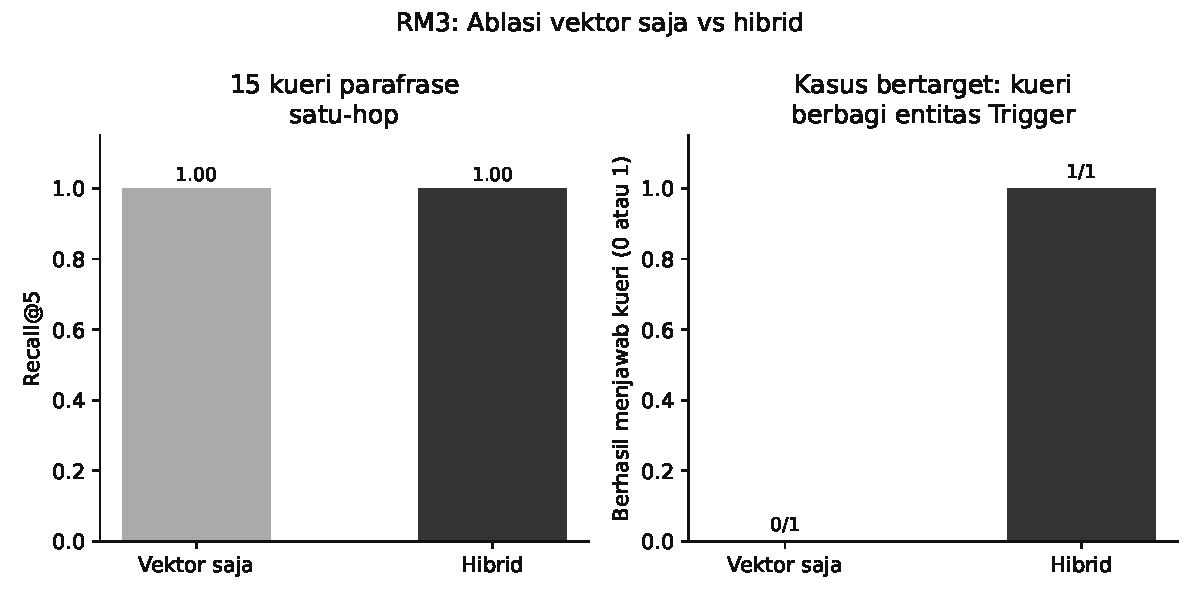
\includegraphics[width=0.9\textwidth]{figures/rm3_ablation_recall.pdf}
  \caption[Recall@5 dan kasus bertarget RM3]{\textit{Recall@5} pada 15 kueri parafrase (kiri) dan keberhasilan kasus bertarget kueri berbagi entitas Trigger (kanan), dari data pada Tabel~\ref{tab:v2-ablation-result}.}
  \label{fig:rm3-ablation-recall}
\end{figure}

\subsubsection{Analisis Hasil Ablasi}

Pada 15 kueri parafrase satu \textit{hop} (satu fakta domain per kueri, kata kueri sengaja tidak mengulang kata pada memori asal), kedua kondisi mencapai \textit{Recall@5} yang sama, yaitu 1,00. Selisih berpasangan bernilai nol pada setiap kueri, sehingga interval kepercayaan 95\% berbasis \textit{bootstrap} (10.000 \textit{resample}) juga degenerasi menjadi [0,00; 0,00]; ini bukan kesalahan perhitungan, melainkan konsekuensi langsung dari kedua kondisi yang benar-benar identik pada setiap kueri probe ini. Temuan ini konsisten dengan sifat kueri yang diuji: parafrase satu \textit{hop} dapat dijawab pencarian kemiripan semantik saja tanpa memerlukan penelusuran relasi graf, sehingga probe ini belum mampu mengisolasi nilai tambah representasi graf terhadap pencarian semantik semata.

Untuk mengisolasi nilai tambah tersebut secara lebih langsung, disusun satu kasus bertarget: dua pengalaman milik pengguna yang sama dibuat berbagi satu entitas Pemicu yang identik pada graf, tetapi kalimatnya sengaja dibuat tidak berbagi kata maupun makna semantik permukaan (satu bercerita tentang tekanan dari dosen pembimbing, satu lagi bercerita tentang liburan ke pantai bersama teman kos, dengan Pemicu yang sama-sama tercatat sebagai relasi terhadap dosen pembimbing tersebut). Pencarian kemiripan semantik hanya menemukan pengalaman pertama; kondisi hibrid berhasil ikut menyertakan pengalaman kedua karena penelusuran satu langkah tambahan pada entitas Pemicu yang sama, mengoperasionalkan prinsip \textit{spreading activation} \parencite{collinsloftus1975} bahwa pengaktifan memori dapat menyebar melalui simpul yang terhubung, bukan hanya melalui kemiripan kata. Kasus tunggal ini tidak memberikan kekuatan statistik, tetapi menunjukkan secara konkret jenis kueri yang secara struktural tidak dapat dijawab pencarian semantik saja, terlepas dari seberapa besar korpus atau seberapa baik model \textit{embedding} yang dipakai.

P@5, MRR, dan nDCG@5 tersedia pada kalibrasi LongMemEval\_S di Tabel~\ref{tab:v2-memory-result}, tetapi tidak dibandingkan antar-kondisi karena korpus tersebut belum dianotasi sebagai graf AXIS. \textit{Update correctness}, \textit{grounded-answer rate}, \textit{false-personalization rate}, dan \textit{stale-belief rate} tidak dibandingkan antara kondisi vektor-saja dan hibrid pada blok ablasi ini karena diukur melalui skenario terpisah (Subbab~\ref{sec:v2-memory}), bukan sebagai perbandingan berpasangan kedua kondisi retrieval. \textit{Stale-memory rate} (peluang \textit{retrieval} memori tidak aktif) tetap belum diukur pada kondisi manapun. Klaim keunggulan kondisi hibrid pada tahap ini dibatasi pada kemampuan menjawab kueri yang mengandalkan identitas relasi graf, bukan pada seluruh kemampuan memori jangka panjang secara umum. Bukti kontrak lifecycle dan probe reappraisal dilaporkan terpisah karena keduanya menguji transisi memori, bukan membandingkan kedua kondisi retrieval.

\section{Validasi Kebutuhan Pendukung Kendali Pengguna}
\label{sec:v2-user-control}

Kendali pengguna tidak diperlakukan sebagai rumusan masalah terpisah. Seluruh kontrol pengguna yang dirancang pada purwarupa telah tersedia pada antarmuka dan dapat digunakan untuk mengelola memori, riwayat percakapan, data pribadi, serta preferensi pengalaman. Verifikasi teknis dilakukan melalui tugas melihat, mengoreksi, menghapus, dan menyembunyikan memori; mengunduh data; menghapus riwayat; menghapus akun; dan memastikan isi \textit{Confession Space} tidak masuk ke memori jangka panjang. Keberhasilan dan kegagalan setiap tugas diverifikasi lewat eksekusi teknis langsung terhadap setiap kontrol. Evaluasi terhadap pemahaman dan kenyamanan pengguna dalam memakai kontrol tersebut tetap menjadi bagian pengujian pengguna nyata (Subbab~\ref{sec:evaluasi-pengguna}).

\begin{table}[!htbp]
\centering
\caption{Hasil validasi kendali pengguna}
\label{tab:v2-user-control}
{\footnotesize
\begin{tabularx}{\textwidth}{|>{\raggedright\arraybackslash}X|>{\centering\arraybackslash}p{1.8cm}|>{\centering\arraybackslash}p{1.8cm}|>{\centering\arraybackslash}p{2.3cm}|}
\hline
\rowcolor{tableheadgray}
\textbf{Tugas} & \textbf{Berhasil} & \textbf{Gagal} & \textbf{Pemahaman pengguna} \\
\hline
Melihat dan mengoreksi memori & 2 & 0 & Memerlukan pengguna nyata \\
\hline
Menghapus atau menyembunyikan memori & 1 & 0 & Memerlukan pengguna nyata \\
\hline
Hapus riwayat percakapan (tingkat sesi) & 1 & 0 & Memerlukan pengguna nyata \\
\hline
Unduh data & 2 & 0 & Memerlukan pengguna nyata \\
\hline
Hapus akun & 2 & 0 & Memerlukan pengguna nyata \\
\hline
Memahami batas persistensi \textit{Confession Space} & 2 & 0 & Memerlukan pengguna nyata \\
\hline
\end{tabularx}
}
\end{table}

Lima dari enam tugas kini memiliki verifikasi teknis otomatis terhadap lapisan layanan produksi: melihat, mengoreksi, dan menyembunyikan (mengarsipkan) satu node memori terverifikasi langsung terhadap layanan memori pada \textit{gateway}; hapus riwayat percakapan tingkat sesi terverifikasi lewat fungsi penghapusan sesi produksi; batas persistensi \textit{Confession Space} terverifikasi lewat mekanisme pengecualian baris aktivitas yang memicu penulisan memori (lihat Tabel~\ref{tab:v2-fungsional} untuk rincian dan batas cakupannya). Tugas mengunduh data diimplementasikan sepenuhnya pada sisi antarmuka: data percakapan pengguna diambil dari titik akhir yang sudah ada, digabungkan menjadi satu berkas, lalu diunduh langsung dari peramban, tanpa titik akhir ekspor khusus pada lapisan \textit{backend}. Implementasi ini terverifikasi berfungsi pada purwarupa yang dideploy (Subbab~\ref{sec:implementasi-arsitektur-inti}). Kolom pemahaman pengguna pada seluruh baris tetap secara struktural memerlukan partisipan nyata dan tidak dapat diisi lewat verifikasi teknis.

\section{Pengendalian Keterulangan dan Pelaporan}
\label{sec:v2-reproducibility}

Setiap eksperimen mencatat penyedia, nama dan snapshot model, tanggal eksekusi, model embedding, temperatur, \textit{top-p}, seed bila tersedia, batas token, versi prompt, snapshot korpus, versi fixture, kondisi cache, dan artefak keluaran. Bila penyedia tidak menyediakan seed atau snapshot tetap, respons dibekukan sebelum anotasi dan keterbatasan tersebut dicatat.

Pelaporan mengikuti aturan berikut:

\begin{enumerate}[label=\arabic*.,leftmargin=*,itemsep=3pt]
  \item tampilkan jumlah kasus dan distribusi label;
  \item tampilkan metrik agregat dan metrik per slice yang relevan;
  \item sertakan interval kepercayaan untuk perbandingan dan kesesuaian;
  \item laporkan konfigurasi model penilai dan rubrik yang digunakan;
  \item simpan matriks kebingungan atau keluaran per kasus sebagai artefak audit;
  \item pisahkan klaim validitas rekayasa dari klaim klinis.
\end{enumerate}

\section{Rencana Evaluasi Lanjutan Pengujian Pengguna Nyata}
\label{sec:evaluasi-pengguna}

Blok ini menjawab aspek yang secara struktural tidak dapat diukur oleh validasi kontrak, \textit{benchmark} berlabel, maupun penilaian buta \textit{LLM-as-judge}, karena ketiganya menilai keluaran sistem terhadap acuan atau rubrik, bukan pengalaman subjektif pengguna itu sendiri. Pengujian pengguna nyata ditujukan untuk mengumpulkan persepsi kegunaan dan rasa didampingi pada RM1 (Subbab~\ref{sec:tujuan} butir 1), kejelasan penyampaian mood dan PHQ-9 pada RM2, serta pemahaman pengguna terhadap konsekuensi tiap kontrol memori pada RM3 (Tabel~\ref{tab:v2-user-control}).

\subsection{Metode Evaluasi}

Partisipan adalah mahasiswa aktif Indonesia yang direkrut secara sukarela, memakai AXIS sekurang-kurangnya 14 hari agar melewati satu siklus penuh penawaran PHQ-9 (D3 pada instrumen), sebelum mengisi kuesioner daring pada Lampiran~\ref{lamp:userstudy}. Purwarupa dapat diakses langsung melalui domain publik yang sudah dideploy (Subbab~\ref{sec:implementasi-arsitektur-inti}), sehingga perekrutan tidak memerlukan distribusi berkas instalasi atau konfigurasi jaringan tambahan kepada partisipan. Kuesioner terdiri atas enam bagian dan 27 butir dengan estimasi pengisian 6--8 menit: profil partisipan, \textit{System Usability Scale} (SUS), persepsi kualitas interaksi dan kesinambungan memori, kejelasan mood/PHQ-9, perbandingan dengan \textit{chatbot} AI umum, dan pengalaman keseluruhan beserta pertanyaan terbuka. Data yang dapat diperoleh otomatis dari sistem (durasi sesi, skor PHQ-9) tidak ditanyakan ulang, sehingga kuesioner murni menangkap persepsi yang tidak dapat diukur dari sisi sistem.

\subsection{Rencana Pengolahan Hasil}

Data kuantitatif (skor SUS, item Likert) dilaporkan secara deskriptif beserta interval kepercayaan 95\% ketika ukuran sampel memadai. Jawaban terbuka dianalisis melalui pengodean tematik, dengan tema yang muncul dilaporkan beserta jumlah partisipan yang menyebutkannya. Hasil dipisahkan menurut moderator D2 (pengalaman \textit{chatbot} AI sebelumnya) dan D3 (durasi penggunaan) agar perbedaan persepsi akibat \textit{familiarity} tidak tercampur dengan perbedaan akibat kualitas sistem itu sendiri. Seluruh hasil dilaporkan sebagai bukti validitas rekayasa dan persepsi awal pengguna, bukan sebagai klaim efektivitas klinis.

\begin{table}[!htbp]
\centering
\caption{Ringkasan hasil pengujian pengguna nyata}
\label{tab:v2-user-study}
{\footnotesize
\begin{tabularx}{\textwidth}{|>{\raggedright\arraybackslash}X|>{\centering\arraybackslash}p{2.8cm}|>{\raggedright\arraybackslash}p{3.2cm}|}
\hline
\rowcolor{tableheadgray}
\textbf{Aspek} & \textbf{Hasil kuantitatif} & \textbf{Temuan kualitatif} \\
\hline
Kegunaan & & \\
\hline
Kualitas interaksi & & \\
\hline
Kejelasan PHQ-9 & & \\
\hline
Kesinambungan memori & & \\
\hline
Keselamatan dan batas peran & & \\
\hline
Kendali data & & \\
\hline
\end{tabularx}
}
\end{table}

\section{Diskusi terhadap Rumusan Masalah}
\label{sec:diskusi-hasil}

\subsection{RM1: Respons Empatik, Relevan, Reflektif, Aman, dan Sesuai Ragam Bahasa}

Tiga blok bukti mendukung RM1 secara terpisah. Penilaian buta pada 24 skenario satu-giliran (Subbab~\ref{sec:v2-dialogue}) menunjukkan AXIS dipilih pada 14 dari 24 penilaian berpasangan menurut konfigurasi penilai primer. Perbedaannya terutama muncul pada kondisi bermemori: AXIS dipilih delapan dari 10 kali, sedangkan pada 14 kondisi tanpa memori, \textit{baseline} sedikit lebih sering dipilih (tujuh berbanding enam). Jadi, klaim yang dapat dipertanggungjawabkan dari blok ini terbatas pada pemanfaatan memori personal, bukan keunggulan kualitas percakapan secara umum. Kesepakatan preferensi antara dua konfigurasi penilai independen pada blok ini rendah (Cohen's kappa $-0,035$), jauh di bawah blok evaluasi lain, sehingga angka preferensi di atas perlu dibaca sebagai hasil satu konfigurasi penilai, bukan kesimpulan yang stabil antarpenilai. Benchmark keselamatan pada korpus 50 pesan (Subbab~\ref{sec:v2-safety}) menghasilkan sensitivitas 0,654, spesifisitas 0,917, dan sembilan \textit{false negative}; semua respons setelah deteksi memenuhi rubrik aman. Dengan demikian, keluaran eskalasi bekerja konsisten pada kasus yang tertangkap, tetapi kemampuan mendeteksi eufemisme masih terbatas. Evaluasi ragam formal dan bahasa campur kini juga diuji pada rubrik respons suportif (lima dan enam skenario secara berurutan), dengan preferensi AXIS setara pada formal dan tertinggal pada bahasa campur; ragam eufemistik hanya didukung satu skenario pada rubrik ini sehingga belum dapat digeneralisasi.

\subsection{RM2: Mood Harian dan Asesmen Skrining Depresi secara Percakapan}

Fidelity orkestrasi PHQ-9 (Subbab~\ref{sec:v2-phq}) lulus penuh pada 130 kontrak suite otomatis yang mencakup penawaran, pemicu onboarding, penyampaian item, klarifikasi, penskoran, umpan balik, dan rute item kesembilan. Mood harian dicatat satu kali per hari dan pemisahan data administratif dilindungi oleh kontrak memori. Pemetaan jawaban bebas ke skor menunjukkan kesepakatan sempurna dengan label acuan pada 73 dari 80 kasus dengan frekuensi tegas; tujuh kasus ambigu secara tepat memicu klarifikasi alih-alih skor paksa. Kesimpulan RM2 pada tahap ini dibatasi pada fidelity penyampaian dan ketepatan pemetaan jawaban bebas skala kecil, tidak diperluas menjadi klaim diagnosis atau efektivitas klinis.

\subsection{RM3: Memori Jangka Panjang yang Berkesinambungan}

Ablasi kondisi vektor saja berbanding hibrid (Subbab~\ref{sec:v2-ablation}) menunjukkan \textit{Recall@5} yang identik (1,00) pada kueri parafrase satu-\textit{hop}, tetapi kondisi hibrid berhasil menjawab kasus bertarget yang secara struktural tidak dapat dijawab pencarian semantik saja (dua pengalaman berbagi identitas simpul Pemicu yang sama tanpa kesamaan leksikal maupun semantik permukaan). Nilai graf pada tahap ini dinyatakan spesifik untuk kemampuan menjawab kueri berbasis identitas relasi, bukan untuk seluruh kemampuan memori jangka panjang. Ketepatan penulisan node (presisi 0,69, \textit{recall} 0,75) dan \textit{update correctness} (0,75) telah diukur melalui teknik pengujian skenario-dan-hasil karena tidak ada korpus publik berbahasa Indonesia yang sesuai. Penggunaan memori pada jawaban (\textit{grounded-answer rate} 1,00, \textit{false-personalization rate} 0,00, dan \textit{stale-belief rate} 0,00) telah diukur melalui teknik serupa (artefak \textit{evaluasi\_v3}), tetapi tetap merupakan proksi skenario berukuran kecil, bukan estimasi populasi.
